% answers.tex —— 2024 年·新高考Ⅱ卷 · 参考答案与详细解析片段
% 由 tools/generate_projects.py 依来源总账自 2024/2024_数学真题_新高考Ⅱ_试题.md + 2024/2024_数学真题_新高考Ⅱ_解析正文.md + 2024/2024_数学真题_新高考Ⅱ_答案要点.md 生成，勿手改（改源 MD 后重跑）


\begin{gknotice}
\textbf{来源说明}：试题原文取自 deekur/gaokaomath（commit \texttt{34c13a6}，CC BY 4.0）之「2024新高考2」PDF，逐题照图转录。

\textbf{解析归属}：本文档全部解析由本库编写者根据试题独立推导，\textbf{非官方标准答案}。推导过程完整给出以便核验；若与官方发布版本不一致，以官方为准。

\textbf{卷种提示}：2024 年是题型分水岭（19 题制），结构与 2025、2026 一致，是最贴近 2027 高考的对标真题之一。
\end{gknotice}

\par\medskip

\gkpart{一、单选题（每小题 5 分，共 40 分）}

\begin{answer}
\gksolhead{1}{}

\textbf{题目}：

已知 $z=-1-\mathrm i$，则 $|z|=$（　　）

\begin{gkopts}(4)
\task A．$0$
\task B．$1$
\task C．$\sqrt2$
\task D．$2$
\end{gkopts}

\textbf{解析}

复数 $z=a+b\mathrm i$ 的模就是它在复平面内对应点 $(a,b)$ 到原点的距离：
\[|z|=\sqrt{a^{2}+b^{2}}\]

本题 $a=-1$，$b=-1$：
\[|z|=\sqrt{(-1)^{2}+(-1)^{2}}=\sqrt{1+1}=\sqrt2\]

\begin{gktip}
\textbf{易错点}：模是\textbf{平方和}开根，与两个负号无关。若把 $-1-\mathrm i$ 的模误算成 $|-1|+|-1|=2$（选 D）或只看实部得 $1$（选 B），都是没有回到定义。
\end{gktip}

\gkanswer{答案：C（$\sqrt2$）}

\par\medskip

\end{answer}
\begin{answer}
\gksolhead{2}{}

\textbf{题目}：

已知命题 $p$：$\forall x\in\mathbf R$，$|x+1|>1$；命题 $q$：$\exists x>0$，$x^{3}=x$。则（　　）

\begin{gkopts}(2)
\task A．$p$ 和 $q$ 都是真命题
\task B．$\neg p$ 和 $q$ 都是真命题
\task C．$p$ 和 $\neg q$ 都是真命题
\task D．$\neg p$ 和 $\neg q$ 都是真命题
\end{gkopts}

\textbf{解析}

\textbf{判断 $p$（全称命题）：只需找一个反例即可否定。}

取 $x=-1$：
\[|(-1)+1|=|0|=0\not>1\]

反例存在，故 $p$ 为\textbf{假命题}，$\neg p$ 为真命题。

\textbf{判断 $q$（存在性命题）：只需找一个例子即可肯定。}

解方程 $x^{3}=x$，即 $x\left(x^{2}-1\right)=0$，得 $x=0,\ 1,\ -1$。其中 $x=1>0$ 满足条件。

故 $q$ 为\textbf{真命题}。

综上，$\neg p$ 和 $q$ 都是真命题。

\begin{gktip}
\textbf{方法总结}：全称命题「$\forall$」与存在性命题「$\exists$」的判断成本完全不对称——\textbf{否定全称、肯定存在都只需举一个例子}；反过来（肯定全称、否定存在）才需要一般性证明。做这类题第一反应应该是「先试特殊值」，本题两个命题都在一步之内定性。
\end{gktip}

\gkanswer{答案：B（$\neg p$ 和 $q$ 都是真命题）}

\par\medskip

\end{answer}
\begin{answer}
\gksolhead{3}{}

\textbf{题目}：

已知向量 $\boldsymbol a$，$\boldsymbol b$ 满足 $|\boldsymbol a|=1$，$|\boldsymbol a+2\boldsymbol b|=2$，且 $(\boldsymbol b-2\boldsymbol a)\perp\boldsymbol b$，则 $|\boldsymbol b|=$（　　）

\begin{gkopts}(2)
\task A．$\dfrac12$
\task B．$\dfrac{\sqrt2}2$
\task C．$\dfrac{\sqrt3}2$
\task D．$1$
\end{gkopts}

\textbf{解析}

\textbf{核心手法：一切条件都平方或化成数量积，把 $\boldsymbol a\cdot\boldsymbol b$ 当作一个整体消掉。}

\textbf{第一步，由垂直条件解出 $\boldsymbol a\cdot\boldsymbol b$。}
\[(\boldsymbol b-2\boldsymbol a)\cdot\boldsymbol b=0\ \Longrightarrow\ |\boldsymbol b|^{2}-2\,\boldsymbol a\cdot\boldsymbol b=0\ \Longrightarrow\ \boldsymbol a\cdot\boldsymbol b=\frac{|\boldsymbol b|^{2}}2\]

\textbf{第二步，把模长条件平方。}
\[|\boldsymbol a+2\boldsymbol b|^{2}=|\boldsymbol a|^{2}+4\,\boldsymbol a\cdot\boldsymbol b+4|\boldsymbol b|^{2}=4\]

\textbf{第三步，代入并整理。}
\[1+4\cdot\frac{|\boldsymbol b|^{2}}2+4|\boldsymbol b|^{2}=4\]
\[1+2|\boldsymbol b|^{2}+4|\boldsymbol b|^{2}=4\ \Longrightarrow\ 6|\boldsymbol b|^{2}=3\ \Longrightarrow\ |\boldsymbol b|^{2}=\frac12\]

\[|\boldsymbol b|=\frac{\sqrt2}2\]

\begin{gktip}
\textbf{一致性自检}（取具体向量验证）：令 $\boldsymbol a=(1,0)$，由 $\boldsymbol a\cdot\boldsymbol b=\dfrac{|\boldsymbol b|^{2}}2=\dfrac14$ 知 $\boldsymbol b=\left(\dfrac14,\ t\right)$，再由 $|\boldsymbol b|^{2}=\dfrac12$ 得 $t^{2}=\dfrac12-\dfrac1{16}=\dfrac7{16}$。此时
\[|\boldsymbol a+2\boldsymbol b|=\left|\left(\frac32,\ 2t\right)\right|=\sqrt{\frac94+\frac74}=\sqrt4=2\quad\checkmark\]
三个条件全部吻合。
\end{gktip}

\gkanswer{答案：B（$\dfrac{\sqrt2}2$）}

\par\medskip

\end{answer}
\begin{answer}
\gksolhead{4}{}

\textbf{题目}：

某农业研究部门在面积相等的 $100$ 块稻田上种植一种新型水稻，得到各块稻田的亩产量（单位：kg）并整理得下表：

\begin{center}
\begin{tabular}{cccc}
\toprule
亩产量 & $[900,950)$ & $[950,1000)$ & $[1000,1050)$ \\
\midrule
频数 & $6$ & $12$ & $18$ \\
\bottomrule
\end{tabular}
\end{center}

\begin{center}
\begin{tabular}{cccc}
\toprule
亩产量 & $[1050,1100)$ & $[1100,1150)$ & $[1150,1200)$ \\
\midrule
频数 & $30$ & $24$ & $10$ \\
\bottomrule
\end{tabular}
\end{center}

  根据表中数据，下列结论中正确的是（　　）

\begin{gkopts}(1)
\task A．$100$ 块稻田亩产量的中位数小于 $1050$ kg
\task B．$100$ 块稻田中亩产量低于 $1100$ kg 的稻田所占比例超过 $80\%$
\task C．$100$ 块稻田亩产量的极差介于 $200$ kg 至 $300$ kg 之间
\task D．$100$ 块稻田亩产量的平均值介于 $900$ kg 至 $1000$ kg 之间
\end{gkopts}

\textbf{解析}

\textbf{基础工作：先把累计频数算出来}（频数分布表的题，累计频数一列能同时解决中位数与比例两类问题）。

\begin{center}
\begin{tabular}{lcccccc}
\toprule
区间 & $[900,950)$ & $[950,1000)$ & $[1000,1050)$ & $[1050,1100)$ & $[1100,1150)$ & $[1150,1200)$ \\
\midrule
频数 & $6$ & $12$ & $18$ & $30$ & $24$ & $10$ \\
累计 & $6$ & $18$ & $36$ & $66$ & $90$ & $100$ \\
\bottomrule
\end{tabular}
\end{center}

总数 $6+12+18+30+24+10=100$ 

\par\medskip

\textbf{A 项}：中位数是第 $50$、$51$ 个数据的平均。累计到 $1050$ 只有 $36$ 个（$<50$），累计到 $1100$ 有 $66$ 个（$>51$），故中位数落在区间 $[1050,1100)$ 内，\textbf{不小于 $1050$}  \textbf{错误}。

\par\medskip

\textbf{B 项}：亩产量低于 $1100$ kg 的共 $66$ 块，占比 $66\%$，\textbf{未超过 $80\%$}  \textbf{错误}。

\par\medskip

\textbf{C 项}：最小值落在 $[900,950)$ 内、最大值落在 $[1150,1200)$ 内，故极差 $R=\max-\min$ 满足
\[R>1150-950=200,\qquad R<1200-900=300\]

即 $R\in(200,300)$  \textbf{正确}。

\par\medskip

\textbf{D 项}：用\textbf{组下限}代替组内数据（这样算出的是平均值的最小可能值）：
\[\bar x>\frac{900\times6+950\times12+1000\times18+1050\times30+1100\times24+1150\times10}{100}\]
\[=\frac{5400+11400+18000+31500+26400+11500}{100}=\frac{104200}{100}=1042\]

平均值\textbf{必大于 $1042$}，远超 $1000$  \textbf{错误}。

（若按组中值估计，$\bar x\approx1067$，同样落在 $[1050,1100)$ 附近。）

\begin{gktip}
\textbf{方法总结}：分组数据题的四个常考量各有各的「只看一处」技巧——\textbf{中位数看累计频数跨过 $50\%$ 的那一组}、\textbf{比例直接读累计}、\textbf{极差用两端组的端点作上下夹逼}、\textbf{平均值用组下限/组上限先做粗估}。四项里只有 D 需要真动手算，而且用下限一次就否掉了，无需精确求平均。
\end{gktip}

\gkanswer{答案：C（极差介于 $200$ 至 $300$ kg 之间）}

\par\medskip

\end{answer}
\begin{answer}
\gksolhead{5}{}

\textbf{题目}：

已知曲线 $C:x^{2}+y^{2}=16\ (y>0)$，从 $C$ 上任意一点 $P$ 向 $x$ 轴作垂线段 $PP'$，$P'$ 为垂足，则线段 $PP'$ 的中点 $M$ 的轨迹方程为（　　）

\begin{gkopts}(2)
\task A．$\dfrac{x^{2}}{16}+\dfrac{y^{2}}4=1\ (y>0)$
\task B．$\dfrac{x^{2}}{16}+\dfrac{y^{2}}8=1\ (y>0)$
\task C．$\dfrac{y^{2}}{16}+\dfrac{x^{2}}4=1\ (y>0)$
\task D．$\dfrac{y^{2}}{16}+\dfrac{x^{2}}8=1\ (y>0)$
\end{gkopts}

\textbf{解析}

\textbf{通法：相关点法（代入法）——把「主动点」的坐标用「被动点」表示，再回代已知曲线。}

设 $P\left(x_0,y_0\right)$ 在 $C$ 上，则
\[x_0^{2}+y_0^{2}=16,\qquad y_0>0\]

$PP'\perp x$ 轴，故垂足 $P'\left(x_0,0\right)$，中点
\[M=\left(\frac{x_0+x_0}2,\ \frac{y_0+0}2\right)=\left(x_0,\ \frac{y_0}2\right)\]

设 $M(x,y)$，则
\[x=x_0,\qquad y=\frac{y_0}2\ \Longrightarrow\ x_0=x,\quad y_0=2y\]

\textbf{回代原曲线方程}：
\[x^{2}+(2y)^{2}=16\ \Longrightarrow\ x^{2}+4y^{2}=16\]

两边除以 $16$：
\[\frac{x^{2}}{16}+\frac{y^{2}}4=1\]

又 $y_0>0\iff y>0$。

\begin{gktip}
\textbf{易错点}：两处。其一，别把 $y=\dfrac{y_0}2$ 反解错方向（写成 $y_0=\dfrac y2$ 会得到 $\dfrac{x^2}{16}+4y^2=1$，四个选项里都没有，反而容易发现；但若粗心写成除以 $4$ 就会误选 B）。其二，\textbf{范围条件必须跟着走}：原曲线是上半圆，轨迹也只能是上半椭圆，$y>0$ 不能丢。
\end{gktip}

\gkanswer{答案：A（$\dfrac{x^{2}}{16}+\dfrac{y^{2}}4=1,\ y>0$）}

\par\medskip

\end{answer}
\begin{answer}
\gksolhead{6}{}

\textbf{题目}：

设函数 $f(x)=a(x+1)^{2}-1$，$g(x)=\cos x+2ax$。当 $x\in(-1,1)$ 时，曲线 $y=f(x)$ 与 $y=g(x)$ 恰有一个交点。则 $a=$（　　）

\begin{gkopts}(4)
\task A．$-1$
\task B．$\dfrac12$
\task C．$1$
\task D．$2$
\end{gkopts}

\textbf{解析}

\textbf{第一步，作差，观察结构。} 交点个数 $=$ 差函数的零点个数。令
\[h(x)=f(x)-g(x)=a(x+1)^{2}-1-\cos x-2ax\]

展开 $a(x+1)^{2}=ax^{2}+2ax+a$，\textbf{含 $2ax$ 的项恰好抵消}：
\[h(x)=ax^{2}+2ax+a-1-\cos x-2ax=ax^{2}+a-1-\cos x\]

\[\boxed{h(x)=ax^{2}-\cos x+a-1}\]

\textbf{第二步，发现对称性（本题的题眼）。}

$x^{2}$ 与 $\cos x$ 都是偶函数，故 $h(-x)=h(x)$，即 \textbf{$h$ 是偶函数}；而定义域 $(-1,1)$ 关于原点对称。

于是：若 $x_0\ne0$ 是零点，则 $-x_0$ 也是零点，零点必\textbf{成对出现}。要「恰有一个零点」，这个零点只能是 $x=0$。

\textbf{第三步，由 $h(0)=0$ 定 $a$。}
\[h(0)=0-\cos0+a-1=a-2=0\ \Longrightarrow\ a=2\]

\textbf{第四步，验证充分性}（必要条件求出的值必须回代检验）。

当 $a=2$ 时
\[h(x)=2x^{2}-\cos x+1=2x^{2}+(1-\cos x)\]

对 $x\in(-1,1)$：$1-\cos x\ge0$ 恒成立；当 $x\ne0$ 时 $2x^{2}>0$，故 $h(x)>0$。

因此 $h$ 在 $(-1,1)$ 上\textbf{只有 $x=0$ 一个零点} 

\begin{gktip}
\textbf{方法总结}：「偶函数 + 对称区间 + 恰有一个零点」是一个成套的命题模板，结论永远是「零点必在 $x=0$」，一步就把参数解出来。识别它的关键在于\textbf{先作差再展开}——本题不展开就看不出 $2ax$ 会消掉，也就看不出 $h$ 是偶函数。另外三个选项 $a=-1,\dfrac12,1$ 代入后 $h(0)=a-2\ne0$，此时零点要么成对出现（如 $a=1$ 时有 $x\approx\pm0.824$ 两个）、要么一个也没有。
\end{gktip}

\gkanswer{答案：D（$a=2$）}

\par\medskip

\end{answer}
\begin{answer}
\gksolhead{7}{}

\textbf{题目}：

已知正三棱台 $ABC\text{-}A_1B_1C_1$ 的体积为 $\dfrac{52}3$，$AB=6$，$A_1B_1=2$，则 $A_1A$ 与平面 $ABC$ 所成角的正切值为（　　）

\begin{gkopts}(4)
\task A．$\dfrac12$
\task B．$1$
\task C．$2$
\task D．$3$
\end{gkopts}

\textbf{解析}

\textbf{第一步，用棱台体积公式求高。}

上下底面都是正三角形：
\[S_{\text{\text{下}}}=\frac{\sqrt3}4\times6^{2}=9\sqrt3,\qquad S_{\text{\text{上}}}=\frac{\sqrt3}4\times2^{2}=\sqrt3\]

\[\sqrt{S_{\text{\text{上}}}S_{\text{\text{下}}}}=\sqrt{\sqrt3\times9\sqrt3}=\sqrt{27}=3\sqrt3\]

棱台体积公式：
\[V=\frac h3\left(S_{\text{\text{上}}}+S_{\text{\text{下}}}+\sqrt{S_{\text{\text{上}}}S_{\text{\text{下}}}}\right)=\frac h3\left(\sqrt3+9\sqrt3+3\sqrt3\right)=\frac{13\sqrt3}3h\]

令其等于 $\dfrac{52}3$：
\[\frac{13\sqrt3}3h=\frac{52}3\ \Longrightarrow\ h=\frac{52}{13\sqrt3}=\frac4{\sqrt3}=\frac{4\sqrt3}3\]

\textbf{第二步，找出斜棱在底面上的投影长度。}

正三棱台的两底面中心连线 $O_1O$ 垂直于两底面，$A_1$ 在底面上的射影 $A_1'$ 落在射线 $OA$ 上，且 $OA_1'=R_{\text{\text{上}}}$（上底面外接圆半径）。

正三角形外接圆半径 $=\dfrac{\text{\text{边长}}}{\sqrt3}$：
\[R_{\text{\text{下}}}=\frac6{\sqrt3}=2\sqrt3,\qquad R_{\text{\text{上}}}=\frac2{\sqrt3}=\frac{2\sqrt3}3\]

故投影长度
\[AA_1'=R_{\text{\text{下}}}-R_{\text{\text{上}}}=2\sqrt3-\frac{2\sqrt3}3=\frac{4\sqrt3}3\]

\textbf{第三步，求正切。} 线面角 $\theta=\angle A_1AA_1'$，在直角三角形 $A_1A_1'A$ 中
\[\tan\theta=\frac{A_1A_1'}{AA_1'}=\frac{h}{AA_1'}=\frac{\dfrac{4\sqrt3}3}{\dfrac{4\sqrt3}3}=1\]

\begin{gktip}
\textbf{易错点}：投影距离用的是\textbf{外接圆半径之差}（顶点到中心的距离），不是内切圆半径之差（$\dfrac{\text{\text{边长}}}{2\sqrt3}$），也不是边长之差的一半。判断依据：$A_1A$ 连的是两个\textbf{顶点}，所以要用顶点到中心的距离。用内切圆半径会得到 $AA_1'=\sqrt3-\dfrac{\sqrt3}3=\dfrac{2\sqrt3}3$，$\tan\theta=2$（恰好是干扰项 C）。
\end{gktip}

\gkanswer{答案：B（$1$）}

\par\medskip

\end{answer}
\begin{answer}
\gksolhead{8}{}

\textbf{题目}：

设函数 $f(x)=(x+a)\ln(x+b)$。若 $f(x)\ge0$，则 $a^{2}+b^{2}$ 的最小值为（　　）

\begin{gkopts}(4)
\task A．$\dfrac18$
\task B．$\dfrac14$
\task C．$\dfrac12$
\task D．$1$
\end{gkopts}

\textbf{解析}

\textbf{第一步，把「恒非负」翻译成「两个因子必须同时变号」。}

定义域为 $x+b>0$，即 $x\in(-b,+\infty)$。两个因子各自的符号：

\begin{center}
\begin{tabular}{lccc}
\toprule
因子 & 变号点 & 变号点左侧 & 变号点右侧 \\
\midrule
$\ln(x+b)$ & $x=1-b$ & 负 & 正 \\
$x+a$ & $x=-a$ & 负 & 正 \\
\bottomrule
\end{tabular}
\end{center}

乘积在定义域上恒 $\ge0$，等价于\textbf{两个因子在同一点变号}：

\begin{itemize}
\item 若 $-a<1-b$：取 $x\in(-a,\ 1-b)$，此时 $x+a>0$ 而 $\ln(x+b)<0$，乘积为负，矛盾；
\item 若 $-a>1-b$：取 $x\in(1-b,\ -a)$，此时 $x+a<0$ 而 $\ln(x+b)>0$，乘积为负，矛盾。
\end{itemize}

故必须
\[-a=1-b\ \Longrightarrow\ \boxed{b=a+1}\]

\textbf{第二步，在这条直线上求 $a^{2}+b^{2}$ 的最小值。}

\[a^{2}+b^{2}=a^{2}+(a+1)^{2}=2a^{2}+2a+1=2\left(a+\frac12\right)^{2}+\frac12\ \ge\ \frac12\]

等号在 $a=-\dfrac12$ 时取到，此时 $b=\dfrac12$。

\textbf{第三步，验证取等时确实满足 $f(x)\ge0$。}

$a=-\dfrac12$，$b=\dfrac12$ 时
\[f(x)=\left(x-\frac12\right)\ln\left(x+\frac12\right),\qquad x>-\frac12\]

\begin{itemize}
\item $-\dfrac12<x<\dfrac12$：$x-\dfrac12<0$，$\ln\left(x+\dfrac12\right)<0$，乘积 $>0$ 
\item $x=\dfrac12$：$f=0$ 
\item $x>\dfrac12$：两因子皆正，乘积 $>0$ 
\end{itemize}

\begin{gktip}
\textbf{几何解释}：约束 $b=a+1$ 是 $ab$ 平面上的一条直线，而 $a^{2}+b^{2}$ 是原点到点 $(a,b)$ 距离的平方。所求即\textbf{原点到直线 $b=a+1$（即 $a-b+1=0$）距离的平方}：
\[d=\frac{|0-0+1|}{\sqrt{1^{2}+(-1)^{2}}}=\frac1{\sqrt2}\ \Longrightarrow\ d^{2}=\frac12\]
一步到位，比配方更快。\textbf{看到「线性约束下求平方和最小」，第一反应就该是点到直线距离。}
\end{gktip}

\gkanswer{答案：C（$\dfrac12$）}

\par\medskip

\end{answer}
\gkpart{二、多选题（每小题 6 分，共 18 分）}

\begin{answer}
\gksolhead{9}{}

\textbf{题目}：

对于函数 $f(x)=\sin2x$ 和 $g(x)=\sin\left(2x-\dfrac\pi4\right)$，下列说法中正确的有（　　）

\begin{gkopts}(2)
\task A．$f(x)$ 与 $g(x)$ 有相同的零点
\task B．$f(x)$ 与 $g(x)$ 有相同的最大值
\task C．$f(x)$ 与 $g(x)$ 有相同的最小正周期
\task D．$f(x)$ 与 $g(x)$ 的图象有相同的对称轴
\end{gkopts}

\textbf{解析}

\textbf{关键认识}：$g$ 是把 $f$ 的图象\textbf{向右平移 $\dfrac\pi8$} 得到的（因 $g(x)=\sin2\left(x-\dfrac\pi8\right)$）。平移\textbf{不改变}振幅与周期，但\textbf{会平移}零点与对称轴。四个选项正是按这个分界线设计的。

\par\medskip

\textbf{A 项（零点）}

$f(x)=0\iff2x=k\pi\iff x=\dfrac{k\pi}2$。

$g(x)=0\iff2x-\dfrac\pi4=k\pi\iff x=\dfrac\pi8+\dfrac{k\pi}2$。

两组零点整体相差 $\dfrac\pi8$，无公共元素。最直接的反例：
\[f(0)=\sin0=0,\qquad g(0)=\sin\left(-\frac\pi4\right)=-\frac{\sqrt2}2\ne0\]

 \textbf{错误}。

\par\medskip

\textbf{B 项（最大值）}

$f$、$g$ 都是形如 $\sin(\text{\text{某个一次式}})$ 的函数，其中「某个一次式」都能取遍 $\mathbf R$，故值域都是 $[-1,1]$，最大值都是 $1$  \textbf{正确}。

\par\medskip

\textbf{C 项（最小正周期）}

两者的 $\omega$ 都是 $2$，最小正周期
\[T=\frac{2\pi}{|\omega|}=\frac{2\pi}2=\pi\]

完全相同  \textbf{正确}（相位平移不影响周期）。

\par\medskip

\textbf{D 项（对称轴）}

正弦曲线的对称轴出现在\textbf{取到最值}的位置。

$f$：$2x=\dfrac\pi2+k\pi\Rightarrow x=\dfrac\pi4+\dfrac{k\pi}2$。

$g$：$2x-\dfrac\pi4=\dfrac\pi2+k\pi\Rightarrow x=\dfrac{3\pi}8+\dfrac{k\pi}2$。

两组同样整体相差 $\dfrac\pi8$。反例：$x=\dfrac\pi4$ 是 $f$ 的对称轴（$f=1$ 取到最大值），但
\[g\left(\frac\pi4\right)=\sin\left(\frac\pi2-\frac\pi4\right)=\frac{\sqrt2}2\ne\pm1\]

不是 $g$ 的对称轴  \textbf{错误}。

\begin{gktip}
\textbf{方法总结}：判断两个三角函数「哪些性质相同」，只需分清性质对\textbf{平移}是否敏感：\textbf{振幅、最值、周期、单调区间长度}平移后不变；\textbf{零点、对称轴、对称中心、单调区间的具体位置}平移后整体移动。本题 $g$ 相对 $f$ 右移 $\dfrac\pi8$，于是「不敏感」的 B、C 对，「敏感」的 A、D 错——不必逐个解方程也能秒选。
\end{gktip}

\gkanswer{答案：BC}

\par\medskip

\end{answer}
\begin{answer}
\gksolhead{10}{}

\textbf{题目}：

抛物线 $C:y^{2}=4x$ 的准线为 $l$，$P$ 为 $C$ 上动点。过 $P$ 作 $\odot A:x^{2}+(y-4)^{2}=1$ 的一条切线，$Q$ 为切点。过 $P$ 作 $l$ 的垂线，垂足为 $B$。则（　　）

\begin{gkopts}(1)
\task A．$l$ 与 $\odot A$ 相切
\task B．当 $P$，$A$，$B$ 三点共线时，$|PQ|=\sqrt{15}$
\task C．当 $|PB|=2$ 时，$PA\perp AB$
\task D．满足 $|PA|=|PB|$ 的点 $P$ 有且仅有 $2$ 个
\end{gkopts}

\textbf{解析}

\textbf{基础信息}：$y^{2}=4x$ 中 $2p=4$，故 $p=2$，焦点 $F(1,0)$，准线 $l:x=-1$。$\odot A$ 的圆心 $A(0,4)$，半径 $r=1$。

设 $P\left(x_0,y_0\right)$，则 $y_0^{2}=4x_0$，且垂足 $B\left(-1,\ y_0\right)$，$|PB|=x_0+1$。

\par\medskip

\textbf{A 项}

圆心 $A(0,4)$ 到直线 $x=-1$ 的距离
\[d=|0-(-1)|=1=r\]

恰好等于半径，故 $l$ 与 $\odot A$ \textbf{相切}  \textbf{正确}。

\par\medskip

\textbf{B 项}

$PB\perp l$ 而 $l$ 竖直，故 $PB$ 是\textbf{水平线段}，直线 $PB$ 就是 $y=y_0$。

$P$、$A$、$B$ 三点共线 $\iff$ $A(0,4)$ 也在这条水平线上 $\iff y_0=4$。

此时 $x_0=\dfrac{y_0^{2}}4=4$，即 $P(4,4)$，于是
\[|PA|=\sqrt{(4-0)^{2}+(4-4)^{2}}=4\]

切线长公式（$PQ\perp AQ$，直角三角形 $PQA$）：
\[|PQ|=\sqrt{|PA|^{2}-r^{2}}=\sqrt{16-1}=\sqrt{15}\quad\checkmark\]

 \textbf{正确}。

\par\medskip

\textbf{C 项}

$|PB|=x_0+1=2\Rightarrow x_0=1$，$y_0^{2}=4\Rightarrow y_0=\pm2$。两种情形都要算。

\textbf{情形一}：$P(1,2)$，$B(-1,2)$，$A(0,4)$。
\[\overrightarrow{AP}=(1,-2),\qquad \overrightarrow{AB}=(-1,-2)\]
\[\overrightarrow{AP}\cdot\overrightarrow{AB}=(1)(-1)+(-2)(-2)=-1+4=3\ne0\]

\textbf{情形二}：$P(1,-2)$，$B(-1,-2)$，$A(0,4)$。
\[\overrightarrow{AP}=(1,-6),\qquad \overrightarrow{AB}=(-1,-6)\]
\[\overrightarrow{AP}\cdot\overrightarrow{AB}=-1+36=35\ne0\]

两种情形数量积都不为零，$PA$ 与 $AB$ \textbf{均不垂直}  \textbf{错误}。

\par\medskip

\textbf{D 项}

\textbf{题眼：用抛物线定义把 $|PB|$ 换成 $|PF|$。} $|PB|$ 是 $P$ 到准线的距离，由定义等于 $P$ 到焦点的距离：
\[|PB|=|PF|,\qquad F(1,0)\]

于是
\[|PA|=|PB|\iff|PA|=|PF|\iff P\ \text{\text{在线段}}\ AF\ \text{\text{的中垂线上}}\]

求中垂线：由 $|PA|^{2}=|PF|^{2}$ 得
\[x^{2}+(y-4)^{2}=(x-1)^{2}+y^{2}\]
\[-8y+16=-2x+1\ \Longrightarrow\ 2x=8y-15\ \Longrightarrow\ x=4y-\frac{15}2\]

代入 $y^{2}=4x$：
\[y^{2}=16y-30\ \Longrightarrow\ y^{2}-16y+30=0\]

\[\Delta=16^{2}-4\times30=256-120=136>0\]

有两个不同实根 $y=8\pm\sqrt{34}$，对应 $x=\dfrac{y^{2}}4\ge0$ 自动落在抛物线上。故这样的 $P$ \textbf{恰有 $2$ 个}  \textbf{正确}。

（数值上 $P_1\approx(47.82,\ 13.83)$，$P_2\approx(1.18,\ 2.17)$。）

\begin{gktip}
\textbf{方法总结}：抛物线小题的「万能第一步」是\textbf{把到准线的距离换成到焦点的距离}（或反之）。D 项如果不做这个转化，就要直接联立 $|PA|=x_0+1$ 与 $y_0^2=4x_0$ 解四次式，计算量陡增；转化之后立刻变成「中垂线与抛物线交点个数」，算一个判别式就完。C 项的陷阱则在于 $y_0=\pm2$ \textbf{两个点都得验}——只算一个就下结论是这类题最常见的失分点。
\end{gktip}

\gkanswer{答案：ABD}

\par\medskip

\end{answer}
\begin{answer}
\gksolhead{11}{}

\textbf{题目}：

设函数 $f(x)=2x^{3}-3ax^{2}+1$，则（　　）

\begin{gkopts}(1)
\task A．当 $a>1$ 时，$f(x)$ 有三个零点
\task B．当 $a<0$ 时，$x=0$ 是 $f(x)$ 的极大值点
\task C．存在 $a$，$b$，使得 $x=b$ 为曲线 $y=f(x)$ 的对称轴
\task D．存在 $a$，使得点 $\left(1,f(1)\right)$ 为曲线 $y=f(x)$ 的对称中心
\end{gkopts}

\textbf{解析}

\textbf{基础工作：求导并因式分解。}
\[f'(x)=6x^{2}-6ax=6x(x-a)\]

驻点为 $x=0$ 与 $x=a$，两个关键函数值：
\[f(0)=1,\qquad f(a)=2a^{3}-3a^{3}+1=1-a^{3}\]

\par\medskip

\textbf{A 项}

$a>1>0$，故 $0<a$。$f'$ 的符号：

\begin{center}
\begin{tabular}{lccccc}
\toprule
$x$ & $(-\infty,0)$ & $0$ & $(0,a)$ & $a$ & $(a,+\infty)$ \\
\midrule
$f'(x)$ & $+$ & $0$ & $-$ & $0$ & $+$ \\
$f(x)$ & 增 & 极大 & 减 & 极小 & 增 \\
\bottomrule
\end{tabular}
\end{center}

三次函数（首项系数为正）有三个零点 $\iff$ 极大值 $>0$ 且极小值 $<0$：
\[f(0)=1>0\ \text{（\text{自动成立}）},\qquad f(a)=1-a^{3}<0\iff a^{3}>1\iff a>1\]

条件恰好就是 $a>1$  \textbf{正确}。

\par\medskip

\textbf{B 项}

$a<0$ 时两个驻点的\textbf{大小关系反过来}：$a<0$。重新列表：

\begin{center}
\begin{tabular}{lccccc}
\toprule
$x$ & $(-\infty,a)$ & $a$ & $(a,0)$ & $0$ & $(0,+\infty)$ \\
\midrule
$f'(x)=6x(x-a)$ & $+$ & $0$ & $-$ & $0$ & $+$ \\
$f(x)$ & 增 & 极大 & 减 & 极小 & 增 \\
\bottomrule
\end{tabular}
\end{center}

（验号：在 $(a,0)$ 上 $x<0$ 而 $x-a>0$，乘积为负。）

故 $x=a$ 才是极大值点，$x=0$ 是\textbf{极小值点}  \textbf{错误}。

\par\medskip

\textbf{C 项}

三次函数的首项系数 $2\ne0$，故
\[\lim_{x\to+\infty}f(x)=+\infty,\qquad\lim_{x\to-\infty}f(x)=-\infty\]

若存在对称轴 $x=b$，则恒有 $f(b+t)=f(b-t)$；令 $t\to+\infty$，左端 $\to+\infty$、右端 $\to-\infty$，\textbf{矛盾}  \textbf{错误}。

（更简单的说法：三次函数是\textbf{中心对称}图形，从来不是\textbf{轴对称}图形。）

\par\medskip

\textbf{D 项}

三次函数的对称中心就是它的\textbf{拐点}（二阶导为零处）：
\[f''(x)=12x-6a=0\ \Longrightarrow\ x=\frac a2\]

要使对称中心横坐标为 $1$，取
\[\frac a2=1\ \Longrightarrow\ a=2\]

\textbf{验证} $a=2$：$f(x)=2x^{3}-6x^{2}+1$，$f(1)=2-6+1=-3$。
\[f(1+t)=2(1+t)^{3}-6(1+t)^{2}+1=2t^{3}-6t-3\]
\[f(1-t)=-2t^{3}+6t-3\]
\[f(1+t)+f(1-t)=-6=2f(1)\quad\checkmark\]

确为对称中心  \textbf{正确}。

\begin{gktip}
\textbf{方法总结}：三次函数 $f(x)=Ax^{3}+Bx^{2}+Cx+D\ (A\ne0)$ 有三条「出厂设定」，记住可以秒杀一大类多选题：
1. \textbf{必有对称中心}，横坐标 $x=-\dfrac B{3A}$（即两驻点的中点、也是拐点）；
2. \textbf{必无对称轴}（首尾趋向相反）；
3. \textbf{零点个数}由两个极值的乘积定符号：三个零点 $\iff f(\text{\text{极大}})\cdot f(\text{\text{极小}})<0$。

本题 B 项的陷阱在于 $a<0$ 时两驻点顺序翻转，\textbf{不能沿用 $a>0$ 时画的表}。
\end{gktip}

\gkanswer{答案：AD}

\par\medskip

\end{answer}
\gkpart{三、填空题（每小题 5 分，共 15 分）}

\begin{answer}
\gksolhead{12}{}

\textbf{题目}：

记 $S_n$ 为等差数列 $\left\{a_n\right\}$ 的前 $n$ 项和。若 $a_3+a_4=7$，$3a_2+a_5=5$，则 $S_{10}=$ \gkblank{}．

\textbf{解析}

\textbf{通法：一切化为 $a_1$ 与 $d$。}

\[a_3+a_4=\left(a_1+2d\right)+\left(a_1+3d\right)=2a_1+5d=7\qquad\cdots(1)\]
\[3a_2+a_5=3\left(a_1+d\right)+\left(a_1+4d\right)=4a_1+7d=5\qquad\cdots(2)\]

$(1)\times2-(2)$：
\[\left(4a_1+10d\right)-\left(4a_1+7d\right)=14-5\ \Longrightarrow\ 3d=9\ \Longrightarrow\ d=3\]

代回 $(1)$：
\[2a_1=7-15=-8\ \Longrightarrow\ a_1=-4\]

\textbf{求和}：
\[S_{10}=10a_1+\frac{10\times9}2d=10\times(-4)+45\times3=-40+135=95\]

\begin{gktip}
\textbf{一致性自检}：$d=3$、$a_1=-4$ 时数列为 $-4,-1,2,5,8,11,\cdots$
\[a_3+a_4=2+5=7\ \checkmark,\qquad 3a_2+a_5=3\times(-1)+8=5\ \checkmark\]
\textbf{更快的路线}：$S_{10}=5\left(a_1+a_{10}\right)=5\left(2a_1+9d\right)$。而 $2a_1+9d$ 可由 $(1)$、$(2)$ 直接线性组合出来：$2\times(1)-(2)$ 给出 $3d=9$，再由 $(1)$ 得 $2a_1=-8$，故 $2a_1+9d=-8+27=19$，$S_{10}=5\times19=95$。
\end{gktip}

\gkanswer{答案：$95$}

\par\medskip

\end{answer}
\begin{answer}
\gksolhead{13}{}

\textbf{题目}：

已知 $\alpha$ 为第一象限角，$\beta$ 为第三象限角，$\tan\alpha+\tan\beta=4$，$\tan\alpha\tan\beta=\sqrt2+1$，则 $\sin(\alpha+\beta)=$ \gkblank{}．

\textbf{解析}

\textbf{第一步，整体代入两角和的正切公式}（条件恰好给的是「和」与「积」，不必解出 $\tan\alpha$、$\tan\beta$ 本身）：
\[\tan(\alpha+\beta)=\frac{\tan\alpha+\tan\beta}{1-\tan\alpha\tan\beta}=\frac4{1-\left(\sqrt2+1\right)}=\frac4{-\sqrt2}=-2\sqrt2\]

\textbf{第二步，由正切求正弦的绝对值。}

由 $1+\tan^{2}\theta=\dfrac1{\cos^{2}\theta}$：
\[\cos^{2}(\alpha+\beta)=\frac1{1+8}=\frac19\ \Longrightarrow\ |\cos(\alpha+\beta)|=\frac13\]

\[|\sin(\alpha+\beta)|=\sqrt{1-\frac19}=\frac{2\sqrt2}3\]

\textbf{第三步，定符号（本题真正的考点）。}

由象限条件：
\[\alpha\in\left(2k\pi,\ 2k\pi+\frac\pi2\right),\qquad \beta\in\left(2n\pi+\pi,\ 2n\pi+\frac{3\pi}2\right)\]

两式相加：
\[\alpha+\beta\in\left(2m\pi+\pi,\ 2m\pi+2\pi\right)\qquad(m=k+n)\]

即 $\alpha+\beta$ 落在\textbf{第三或第四象限}，无论哪种情形都有
\[\sin(\alpha+\beta)<0\]

（再结合 $\tan(\alpha+\beta)=-2\sqrt2<0$ 可进一步锁定在第四象限，但求 $\sin$ 的符号已经够用。）

\[\sin(\alpha+\beta)=-\frac{2\sqrt2}3\]

\begin{gktip}
\textbf{数值自检}：$\tan\alpha$、$\tan\beta$ 是方程 $t^{2}-4t+\left(\sqrt2+1\right)=0$ 的两根，约为 $3.2593$ 与 $0.7407$（判别式 $12-4\sqrt2>0$，且两根同为正，与「第一象限角、第三象限角的正切都为正」相符）。取 $\alpha\approx1.2731$、$\beta\approx\pi+0.6376\approx3.7791$，则 $\alpha+\beta\approx5.0522$，$\sin(\alpha+\beta)\approx-0.9428$，而 $-\dfrac{2\sqrt2}3\approx-0.9428$ 

\textbf{易错点}：算出 $\tan(\alpha+\beta)=-2\sqrt2$ 后直接取 $\sin=\dfrac{2\sqrt2}3$（默认落在第二象限）是本题最大的坑。\textbf{只要题目给了象限条件，就一定是用来定符号的}——把 $\alpha$、$\beta$ 的范围相加再看和角落在哪里，是唯一可靠的做法。
\end{gktip}

\gkanswer{答案：$-\dfrac{2\sqrt2}3$}

\par\medskip

\end{answer}
\begin{answer}
\gksolhead{14}{}

\textbf{题目}：

在如图的 $4\times4$ 的方格表中选 $4$ 个方格，要求每行和每列均恰有一个方格被选中，则共有 \gkblank{} 种选法。在所有符合上述要求的选法中，选中方格中的 $4$ 个数之和的最大值是 \gkblank{}．

\begin{center}
\begin{tabular}{cccc}
\toprule
 &  &  &  \\
\midrule
$11$ & $21$ & $31$ & $40$ \\
$12$ & $22$ & $33$ & $42$ \\
$13$ & $22$ & $33$ & $43$ \\
$15$ & $24$ & $34$ & $44$ \\
\bottomrule
\end{tabular}
\end{center}

\textbf{解析}

\textbf{第一空：计数}

「每行恰有一个、每列恰有一个」等价于给第 $1,2,3,4$ 行各指定一个\textbf{互不相同}的列号，也就是 $\{1,2,3,4\}$ 的一个\textbf{排列}：
\[4!=4\times3\times2\times1=24\ \text{\text{种}}\]

\textbf{第二空：最大和}

\textbf{关键观察：把每个数拆成「十位贡献 + 个位贡献」。} 记第 $i$ 行第 $j$ 列的数为 $m_{ij}$，观察到
\[m_{ij}=10j+d_{ij}\]

其中「余项」$d_{ij}$ 构成下表：

\begin{center}
\begin{tabular}{cccccc}
\toprule
行号 & 第 1 列 & 第 2 列 & 第 3 列 & 第 4 列 & 本行最大 \\
\midrule
第 1 行 & $1$ & $1$ & $1$ & $0$ & $1$ \\
第 2 行 & $2$ & $2$ & $3$ & $2$ & $3$ \\
第 3 行 & $3$ & $2$ & $3$ & $3$ & $3$ \\
第 4 行 & $5$ & $4$ & $4$ & $4$ & $5$ \\
\bottomrule
\end{tabular}
\end{center}

\textbf{由于每列恰被选中一次}，所有 $10j$ 的贡献之和是固定的：
\[10\times(1+2+3+4)=100\]

于是
\[\text{\text{总和}}=100+\sum_{i=1}^{4}d_{i,\sigma(i)}\]

只需最大化余项之和。\textbf{先给上界}：每行的余项至多取本行最大值，故
\[\sum d\le1+3+3+5=12\ \Longrightarrow\ \text{\text{总和}}\le112\]

\textbf{再验证上界可达}（必须找出一组互不相同的列）：

\begin{center}
\begin{tabular}{lcccc}
\toprule
选中位置 & 第 4 行第 1 列 & 第 1 行第 2 列 & 第 2 行第 3 列 & 第 3 行第 4 列 \\
\midrule
数值 & $15$ & $21$ & $33$ & $43$ \\
余项 $d$ & $5$ & $1$ & $3$ & $3$ \\
\bottomrule
\end{tabular}
\end{center}

四个列号 $1,2,3,4$ 互不相同 ，四个行号 $4,1,2,3$ 互不相同 ，余项之和 $5+1+3+3=12$ 达到上界。

\[15+21+33+43=112\]

\begin{gktip}
\textbf{方法总结}：这类「每行每列各取一个、求和最大」的题（本质是\textbf{指派问题}）不要盲目枚举 $24$ 种。标准套路两步：
1. \textbf{拆出与选法无关的固定部分}（本题是十位的 $100$），把问题降到更小的数上；
2. \textbf{先按行取最大值得到上界，再构造一组不冲突的位置去够到它}。上界一旦被构造实现，就不必再看其余情形。

若上界够不到（列冲突），则退而求其次逐步调整——本题运气好，一次就命中。
\end{gktip}

\gkanswer{答案：$24$；$112$}

\par\medskip

\end{answer}
\gkpart{四、解答题（共 77 分）}

\begin{answer}
\gksolhead{15}{13 分}

\textbf{题目}（13 分）：

记 $\triangle ABC$ 的内角 $A$，$B$，$C$ 的对边分别为 $a$，$b$，$c$，已知 $\sin A+\sqrt3\cos A=2$。

  (1) 求 $A$；

  (2) 若 $a=2$，$\sqrt2\,b\sin C=c\sin2B$，求 $\triangle ABC$ 的周长。

\textbf{解析}

\par\medskip

\textbf{(1) 解}

\textbf{辅助角公式}：$a\sin\theta+b\cos\theta=\sqrt{a^{2}+b^{2}}\sin(\theta+\varphi)$。这里 $\sqrt{1^{2}+\left(\sqrt3\right)^{2}}=2$：
\[\sin A+\sqrt3\cos A=2\left(\frac12\sin A+\frac{\sqrt3}2\cos A\right)=2\sin\left(A+\frac\pi3\right)\]

由条件
\[2\sin\left(A+\frac\pi3\right)=2\ \Longrightarrow\ \sin\left(A+\frac\pi3\right)=1\]

因 $A\in(0,\pi)$，有 $A+\dfrac\pi3\in\left(\dfrac\pi3,\ \dfrac{4\pi}3\right)$，其中使正弦取 $1$ 的只有
\[A+\frac\pi3=\frac\pi2\ \Longrightarrow\ A=\frac\pi6\]

\textbf{所以 $A=\dfrac\pi6$。}

\par\medskip

\textbf{(2) 解}

\textbf{第一步，化简第二个条件求出 $B$。}

把 $\sin2B=2\sin B\cos B$ 代入：
\[\sqrt2\,b\sin C=2c\sin B\cos B\]

由正弦定理 $b=2R\sin B$、$c=2R\sin C$（$R$ 为外接圆半径）：
\[\sqrt2\cdot2R\sin B\cdot\sin C=2\cdot2R\sin C\cdot\sin B\cos B\]

因 $\sin B>0$、$\sin C>0$，两边可同除以 $2R\sin B\sin C$：
\[\sqrt2=2\cos B\ \Longrightarrow\ \cos B=\frac{\sqrt2}2\]

因 $B\in(0,\pi)$，得
\[B=\frac\pi4\]

\textbf{第二步，求第三个角。}
\[C=\pi-A-B=\pi-\frac\pi6-\frac\pi4=\frac{12\pi-2\pi-3\pi}{12}=\frac{7\pi}{12}\]

\[\sin C=\sin\frac{7\pi}{12}=\sin105^{\circ}=\sin\left(60^{\circ}+45^{\circ}\right)=\frac{\sqrt3}2\cdot\frac{\sqrt2}2+\frac12\cdot\frac{\sqrt2}2=\frac{\sqrt6+\sqrt2}4\]

\textbf{第三步，用正弦定理求三边。}
\[2R=\frac a{\sin A}=\frac2{\sin\dfrac\pi6}=\frac2{\dfrac12}=4\]

\[b=2R\sin B=4\times\frac{\sqrt2}2=2\sqrt2\]
\[c=2R\sin C=4\times\frac{\sqrt6+\sqrt2}4=\sqrt6+\sqrt2\]

\textbf{第四步，求周长。}
\[L=a+b+c=2+2\sqrt2+\sqrt6+\sqrt2=2+3\sqrt2+\sqrt6\]

\textbf{所以 $\triangle ABC$ 的周长为 $2+3\sqrt2+\sqrt6$}（约 $8.69$）。

\begin{gktip}
\textbf{一致性自检}：$b=2\sqrt2\approx2.828$，$c=\sqrt6+\sqrt2\approx3.864$。回代原条件
\[\sqrt2\,b\sin C=\sqrt2\times2\sqrt2\times\sin105^{\circ}=4\times0.9659\approx3.864\]
\[c\sin2B=3.864\times\sin\frac\pi2=3.864\]
两端吻合  且三边满足 $a<b<c$ 与 $A<B<C$ 的对应关系 

\textbf{方法总结}：形如「$\lambda b\sin C=c\sin2B$」的条件，标准动作是\textbf{先把 $\sin2B$ 拆开、再用正弦定理把边全换成角}，两侧的 $\sin B\sin C$ 必然对消，剩下一个只含 $\cos B$ 的方程。\textbf{不要先用余弦定理}——那会引入 $a$，把简单问题复杂化。
\end{gktip}

\gkanswer{答案（1）：$A=\dfrac\pi6$}

\gkanswer{答案（2）：周长 $=2+3\sqrt2+\sqrt6$}

\par\medskip

\end{answer}
\begin{answer}
\gksolhead{16}{15 分}

\textbf{题目}（15 分）：

已知函数 $f(x)=\mathrm e^{x}-ax-a^{3}$。

  (1) 当 $a=1$ 时，求曲线 $y=f(x)$ 在点 $\left(1,f(1)\right)$ 处的切线方程；

  (2) 若 $f(x)$ 有极小值，且极小值小于 $0$，求 $a$ 的取值范围。

\textbf{解析}

\par\medskip

\textbf{(1) 解}

$a=1$ 时
\[f(x)=\mathrm e^{x}-x-1\]

\textbf{切点纵坐标}：
\[f(1)=\mathrm e-1-1=\mathrm e-2\]

\textbf{斜率}：
\[f'(x)=\mathrm e^{x}-1\ \Longrightarrow\ k=f'(1)=\mathrm e-1\]

\textbf{点斜式}：
\[y-(\mathrm e-2)=(\mathrm e-1)(x-1)\]
\[y=(\mathrm e-1)x-(\mathrm e-1)+\mathrm e-2=(\mathrm e-1)x-1\]

\textbf{所以切线方程为 $y=(\mathrm e-1)x-1$。}

（自检：令 $x=1$ 得 $y=\mathrm e-1-1=\mathrm e-2=f(1)$  切线确实过切点。）

\par\medskip

\textbf{(2) 解}

\[f'(x)=\mathrm e^{x}-a\]

\textbf{第一步，先看什么时候才存在极小值。}

\begin{itemize}
\item 若 $a\le0$：$\mathrm e^{x}>0\ge a$，故 $f'(x)>0$ 恒成立，$f$ 在 $\mathbf R$ 上单调递增，\textbf{没有极值}，不合题意。
\item 若 $a>0$：$f'(x)<0\iff x<\ln a$，$f'(x)>0\iff x>\ln a$。故 $f$ 在 $(-\infty,\ln a)$ 递减、在 $(\ln a,+\infty)$ 递增，$x=\ln a$ 是\textbf{唯一的极小值点}。
\end{itemize}

因此必须 $a>0$。

\textbf{第二步，写出极小值并令其小于 $0$。}
\[f(\ln a)=\mathrm e^{\ln a}-a\ln a-a^{3}=a-a\ln a-a^{3}<0\]

\textbf{第三步，除以 $a>0$ 化简}（这一步把三次问题降为可分析的形式）：
\[1-\ln a-a^{2}<0\ \Longleftrightarrow\ a^{2}+\ln a>1\]

\textbf{第四步，用单调性解不等式。}

令
\[\varphi(a)=a^{2}+\ln a,\qquad a>0\]

\[\varphi'(a)=2a+\frac1a>0\]

故 $\varphi$ 在 $(0,+\infty)$ 上\textbf{严格单调递增}；又
\[\varphi(1)=1+\ln1=1\]

于是
\[\varphi(a)>1=\varphi(1)\iff a>1\]

\textbf{所以 $a$ 的取值范围是 $(1,+\infty)$。}

\begin{gktip}
\textbf{一致性自检}：
\begin{itemize}
\item $a=1$（临界）：极小值 $f(0)=1-0-1=0$，恰好\textbf{不小于} $0$，被排除 
\item $a=1.2$：极小值 $f(\ln1.2)\approx-0.747<0$ 
\item $a=0.5$：极小值 $f(\ln0.5)\approx0.722>0$，不合 
\end{itemize}

\textbf{方法总结}：含参极值题的三步骨架——\textbf{① 先讨论极值是否存在（定参数的初步范围）；② 把极值点回代写出极值的解析式；③ 把「极值 $<0$」化成一个单变量不等式，用单调函数 + 特殊点（这里是 $\varphi(1)=1$）一击定界。} 第 ③ 步能否顺利，取决于第 ② 步化简得干不干净——本题除以 $a$ 之后 $a^{2}+\ln a$ 的单调性一目了然，是命题人预留的通道。
\end{gktip}

\gkanswer{答案（1）：$y=(\mathrm e-1)x-1$}

\gkanswer{答案（2）：$a\in(1,+\infty)$}

\par\medskip

\end{answer}
\begin{answer}
\gksolhead{17}{15 分}

\textbf{题目}（15 分）：

如图，平面四边形 $ABCD$ 中，$AB=8$，$CD=3$，$AD=5\sqrt3$，$\angle ADC=90^{\circ}$，$\angle BAD=30^{\circ}$，点 $E$，$F$ 满足 $\overrightarrow{AE}=\dfrac25\overrightarrow{AD}$，$\overrightarrow{AF}=\dfrac12\overrightarrow{AB}$，将 $\triangle AEF$ 沿 $EF$ 翻折至 $\triangle PEF$，使得 $PC=4\sqrt3$。

\begin{center}% 2024 新高考Ⅱ卷 17：矩形沿 EF 翻折后的立体（P 为翻起的 A 点新位置）
% 绘制依据：转录 agent 自源 PDF 逐边核对的构型——立体坐标 E(0,0,0)、D(3√3,0,0)、
% F(0,2,0)、B(2√3,4,0)、C(3√3,3,0)、P(0,0,2√3)，折前 A(-2√3,0,0) 保留示折痕来源；
% 实线 A-E、A-F、F-B、B-C、C-D、P-F、P-B、P-C、P-D，虚线 E-D、E-F、P-E。
% 画布投影：(x,y,z) -> x·(1,0.13) + y·(-0.275,-0.525) + z·(0,0.9)
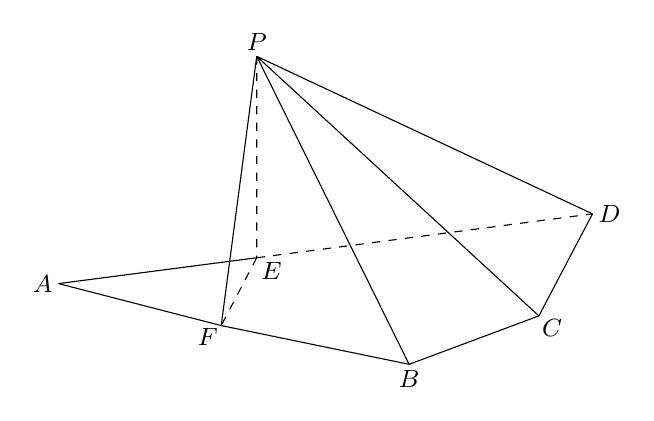
\begin{tikzpicture}[scale=0.82, font=\small]
  \coordinate (A) at (-3.07,-0.40);
  \coordinate (E) at (0,0);
  \coordinate (D) at (5.20,0.68);
  \coordinate (F) at (-0.55,-1.05);
  \coordinate (B) at (2.36,-1.65);
  \coordinate (C) at (4.37,-0.90);
  \coordinate (P) at (0,3.12);
  \draw (A) -- (E)  (A) -- (F);
  \draw (F) -- (B) -- (C) -- (D);
  \draw (P) -- (F)  (P) -- (B)  (P) -- (C)  (P) -- (D);
  \draw[dashed] (E) -- (D)  (E) -- (F)  (P) -- (E);
  \node[left, inner sep=2pt] at (A) {$A$};
  \node[below right, inner sep=1.5pt] at (E) {$E$};
  \node[right, inner sep=2pt] at (D) {$D$};
  \node[below left, inner sep=1pt] at (F) {$F$};
  \node[below, inner sep=2pt] at (B) {$B$};
  \node[below right, inner sep=1pt] at (C) {$C$};
  \node[above, inner sep=2pt] at (P) {$P$};
\end{tikzpicture}\end{center}

  (1) 证明：$EF\perp PD$；

  (2) 求面 $PCD$ 与面 $PBF$ 所成的二面角的正弦值。

\textbf{解析}

\par\medskip

\textbf{预备：在翻折之前把 $\triangle AEF$ 解清楚（两问共用，也是全题的钥匙）}

由分点条件：
\[AE=\frac25AD=\frac25\times5\sqrt3=2\sqrt3,\qquad AF=\frac12AB=\frac12\times8=4\]

夹角 $\angle EAF=\angle BAD=30^{\circ}$。由余弦定理：
\[EF^{2}=AE^{2}+AF^{2}-2\cdot AE\cdot AF\cos30^{\circ}=12+16-2\times2\sqrt3\times4\times\frac{\sqrt3}2=28-24=4\]

\[EF=2\]

\textbf{关键发现}：
\[AE^{2}+EF^{2}=12+4=16=AF^{2}\]

由勾股定理的逆定理，
\[\angle AEF=90^{\circ},\qquad\text{\text{即}}\qquad EF\perp AE\]

而 $E$ 在线段 $AD$ 上，故 $AE$ 与 $ED$ 共线，于是同时有
\[EF\perp ED\]

另记
\[ED=AD-AE=5\sqrt3-2\sqrt3=3\sqrt3\]

\par\medskip

\textbf{(1) 证明}

翻折 $\triangle AEF$ 时，\textbf{折痕 $EF$ 与三角形内部的一切度量关系都不变}，特别地
\[EF\perp EP\qquad(\text{\text{因翻折前} }EF\perp EA,\ \text{\text{而} }EP=EA\text{ \text{是同一条边}})\]

同时，$E$、$D$、$F$ 都在\textbf{不动的底面}上，翻折前已证 $EF\perp ED$，翻折后依然成立：
\[EF\perp ED\]

$EP$ 与 $ED$ 是平面 $PED$ 内两条相交直线（交于 $E$），由\textbf{线面垂直的判定定理}：
\[EF\perp\text{\text{平面} }PED\]

又 $PD\subset$ 平面 $PED$，由线面垂直的性质：
\[EF\perp PD\qquad\blacksquare\]

\begin{gktip}
\textbf{注意}：本问\textbf{完全不需要用到条件 $PC=4\sqrt3$}——它是第 (2) 问用来确定翻折角度的。第 (1) 问对任意翻折角度都成立。
\end{gktip}

\par\medskip

\textbf{(2) 解}

\textbf{第一步，建立坐标系并写出底面各点。}

由 (1)，$EF\perp$ 平面 $PED$。以 $E$ 为原点，$ED$ 方向为 $x$ 轴、$EF$ 方向为 $y$ 轴、与二者都垂直的方向为 $z$ 轴（$P$ 一侧为正）建立空间直角坐标系。底面（即原平面 $ABCD$ 去掉 $\triangle AEF$ 的部分）位于 $z=0$：

\[E(0,0,0),\qquad D\left(3\sqrt3,\ 0,\ 0\right),\qquad F(0,\ 2,\ 0)\]

\textbf{翻折前}的 $A$ 与 $D$ 分居 $E$ 两侧且 $AE=2\sqrt3$，故原位置 $A\left(-2\sqrt3,0,0\right)$。由 $\angle BAD=30^{\circ}$、$AB=8$：
\[B=A+8\left(\cos30^{\circ},\ \sin30^{\circ},\ 0\right)=\left(-2\sqrt3+4\sqrt3,\ 4,\ 0\right)=\left(2\sqrt3,\ 4,\ 0\right)\]

（\textbf{自检}：$F=A+4\left(\cos30^{\circ},\sin30^{\circ},0\right)=\left(-2\sqrt3+2\sqrt3,\ 2,\ 0\right)=(0,2,0)$，与上面写的 $F$ 一致 ）

由 $\angle ADC=90^{\circ}$ 知 $DC\perp DA$；$DA$ 沿 $x$ 轴方向，故 $DC$ 沿 $y$ 轴方向，且 $C$ 与 $B$ 在 $AD$ 同侧（$y>0$），$CD=3$：
\[C=\left(3\sqrt3,\ 3,\ 0\right)\]

\textbf{第二步，用 $PC=4\sqrt3$ 定出 $P$。}

由 (1)，$P$ 在平面 $PED$ 即 $xOz$ 平面内，且 $EP=EA=2\sqrt3$，故可设
\[P=\left(2\sqrt3\cos\theta,\ 0,\ 2\sqrt3\sin\theta\right),\qquad\theta\in(0,\pi)\]

\[PC^{2}=\left(3\sqrt3-2\sqrt3\cos\theta\right)^{2}+3^{2}+\left(2\sqrt3\sin\theta\right)^{2}\]
\[=27-36\cos\theta+12\cos^{2}\theta+9+12\sin^{2}\theta=48-36\cos\theta\]

令 $PC^{2}=\left(4\sqrt3\right)^{2}=48$：
\[48-36\cos\theta=48\ \Longrightarrow\ \cos\theta=0\ \Longrightarrow\ \theta=\frac\pi2\]

\[\boxed{P\left(0,\ 0,\ 2\sqrt3\right)}\]

即翻折到 \textbf{$PE\perp$ 底面}的位置——这是命题人用 $PC=4\sqrt3$ 精心安排的。

\textbf{第三步，求两个平面的法向量。}

\textbf{平面 $PCD$}（过 $P(0,0,2\sqrt3)$、$C\left(3\sqrt3,3,0\right)$、$D\left(3\sqrt3,0,0\right)$）：
\[\overrightarrow{DC}=(0,\ 3,\ 0),\qquad\overrightarrow{DP}=\left(-3\sqrt3,\ 0,\ 2\sqrt3\right)\]

\[\boldsymbol n_1=\overrightarrow{DC}\times\overrightarrow{DP}=\left(3\times2\sqrt3-0,\ \ 0-0,\ \ 0-3\times\left(-3\sqrt3\right)\right)=\left(6\sqrt3,\ 0,\ 9\sqrt3\right)\]

同除以 $3\sqrt3$，取
\[\boldsymbol n_1=(2,\ 0,\ 3),\qquad\left|\boldsymbol n_1\right|=\sqrt{4+9}=\sqrt{13}\]

\textbf{平面 $PBF$}（过 $P(0,0,2\sqrt3)$、$B\left(2\sqrt3,4,0\right)$、$F(0,2,0)$）：
\[\overrightarrow{FB}=\left(2\sqrt3,\ 2,\ 0\right),\qquad\overrightarrow{FP}=\left(0,\ -2,\ 2\sqrt3\right)\]

\[\boldsymbol n_2=\overrightarrow{FB}\times\overrightarrow{FP}=\left(2\times2\sqrt3-0,\,0-2\sqrt3\times2\sqrt3,\,2\sqrt3\times(-2)-0\right)=\left(4\sqrt3,\ -12,\ -4\sqrt3\right)\]

同除以 $4$，取
\[\boldsymbol n_2=\left(\sqrt3,\ -3,\ -\sqrt3\right),\qquad\left|\boldsymbol n_2\right|=\sqrt{3+9+3}=\sqrt{15}\]

\textbf{第四步，求夹角。}
\[\boldsymbol n_1\cdot\boldsymbol n_2=2\times\sqrt3+0\times(-3)+3\times\left(-\sqrt3\right)=2\sqrt3-3\sqrt3=-\sqrt3\]

\[\left|\cos\theta\right|=\frac{\left|\boldsymbol n_1\cdot\boldsymbol n_2\right|}{\left|\boldsymbol n_1\right|\left|\boldsymbol n_2\right|}=\frac{\sqrt3}{\sqrt{13}\times\sqrt{15}}=\frac{\sqrt3}{\sqrt{195}}=\sqrt{\frac3{195}}=\frac1{\sqrt{65}}\]

\[\sin\theta=\sqrt{1-\frac1{65}}=\sqrt{\frac{64}{65}}=\frac8{\sqrt{65}}=\frac{8\sqrt{65}}{65}\]

\textbf{所以面 $PCD$ 与面 $PBF$ 所成二面角的正弦值为 $\dfrac{8\sqrt{65}}{65}$}（约 $0.992$，说明两面几乎垂直）。

\begin{gktip}
\textbf{方法总结}：翻折题的通用流程是\textbf{「折前算清、折后建系」}：
1. \textbf{折前}在平面图形里把与折痕有关的长度、角度全部算出来（本题一算就发现 $\angle AEF=90^{\circ}$，这是全题的题眼）；
2. 由「折痕垂直于两条相交直线」得到\textbf{折痕垂直于某个平面}，第 (1) 问往往到此即止；
3. \textbf{折后}用剩下的那个数量条件（本题是 $PC=4\sqrt3$）把翻折角度解出来，通常会落在「垂直」这种整齐位置；
4. 建系算法向量。

\textbf{易错点}：第 (2) 问设 $P$ 时若忘记「$P$ 必在 $xOz$ 平面内」（这正是第 (1) 问的结论），就会多引入一个未知数、无法求解。\textbf{第 (1) 问的结论要当作第 (2) 问的已知用。}
\end{gktip}

\gkanswer{答案（1）：见解析版}

\gkanswer{答案（2）：$\dfrac{8\sqrt{65}}{65}$}

\par\medskip

\end{answer}
\begin{answer}
\gksolhead{18}{17 分}

\textbf{题目}（17 分）：

某投篮比赛分为两个阶段，每个参赛队由两名队员组成。比赛具体规则如下：第一阶段由参赛队中一名队员投篮 $3$ 次，若 $3$ 次都未投中，则该队被淘汰，比赛成绩为 $0$ 分；若至少投中 $1$ 次，则该队进入第二阶段。第二阶段由该队的另一名队员投篮 $3$ 次，每次投篮投中得 $5$ 分，未投中得 $0$ 分。该队的比赛成绩为第二阶段的得分总和。某参赛队由甲、乙两名队员组成，设甲每次投中的概率为 $p$，乙每次投中的概率为 $q$，各次投中与否相互独立。

  (1) 若 $p=0.4$，$q=0.5$，甲参加第一阶段比赛，求甲、乙所在队的比赛成绩不少于 $5$ 分的概率；

  (2) 假设 $0<p<q$。

  　① 为使得甲、乙所在队的比赛成绩为 $15$ 分的概率最大，应该由谁参加第一阶段比赛？

  　② 为使得甲、乙所在队的比赛成绩的数学期望最大，应该由谁参加第一阶段比赛？

\textbf{解析}

\par\medskip

\textbf{预备：把规则翻译成两个独立事件的乘积}

比赛成绩只由第二阶段决定，而能否进入第二阶段由第一阶段决定，两个阶段相互独立。记
\[A(x)=1-(1-x)^{3}\]
为「命中率为 $x$ 的人投 $3$ 次至少中 $1$ 次」的概率（也就是通过第一阶段的概率）。

展开备用：
\[A(x)=1-\left(1-3x+3x^{2}-x^{3}\right)=3x-3x^{2}+x^{3}=x\left(3-3x+x^{2}\right)\]

\par\medskip

\textbf{(1) 解}

\[\text{\text{成绩}}\ge5\ \text{\text{分}}\iff\text{\text{进入第二阶段，且第二阶段至少投中} }1\ \text{\text{次}}\]

（因为成绩只能是 $0,5,10,15$ 分，$\ge5$ 就等价于「不是 $0$ 分」。而 $0$ 分有两种来源：第一阶段被淘汰，或进入第二阶段但 $3$ 次全不中。）

\textbf{甲通过第一阶段}（$p=0.4$）：
\[A(0.4)=1-(1-0.4)^{3}=1-0.6^{3}=1-0.216=0.784\]

\textbf{乙在第二阶段至少中 $1$ 次}（$q=0.5$）：
\[1-(1-0.5)^{3}=1-0.125=0.875\]

两阶段独立，相乘：
\[P=0.784\times0.875=0.686\]

\textbf{所以所求概率为 $0.686$。}

（$200$ 万次随机模拟得 $0.6861$，与理论值吻合 ）

\par\medskip

\textbf{(2) ① 解}

\textbf{成绩为 $15$ 分 $\iff$ 通过第一阶段，且第二阶段 $3$ 次全中。}

\[P_{\text{\text{甲先}}}=A(p)\cdot q^{3},\qquad P_{\text{\text{乙先}}}=A(q)\cdot p^{3}\]

\textbf{作比较}（两者都为正，作商更清爽）：
\[\frac{P_{\text{\text{甲先}}}}{P_{\text{\text{乙先}}}}=\frac{p\left(3-3p+p^{2}\right)q^{3}}{q\left(3-3q+q^{2}\right)p^{3}}=\frac{\dfrac{3-3p+p^{2}}{p^{2}}}{\dfrac{3-3q+q^{2}}{q^{2}}}\]

\textbf{构造函数}：
\[\psi(x)=\frac{3-3x+x^{2}}{x^{2}}=\frac3{x^{2}}-\frac3x+1,\qquad 0<x\le1\]

（注意分子 $3-3x+x^{2}$ 的判别式 $9-12<0$，故 $\psi(x)>0$ 恒成立。）

\textbf{求导判单调}：
\[\psi'(x)=-\frac6{x^{3}}+\frac3{x^{2}}=\frac{3x-6}{x^{3}}=\frac{3(x-2)}{x^{3}}\]

当 $0<x\le1$ 时 $x-2<0$、$x^{3}>0$，故 $\psi'(x)<0$，$\psi$ \textbf{严格递减}。

由 $0<p<q\le1$：
\[\psi(p)>\psi(q)>0\ \Longrightarrow\ \frac{P_{\text{\text{甲先}}}}{P_{\text{\text{乙先}}}}>1\ \Longrightarrow\ P_{\text{\text{甲先}}}>P_{\text{\text{乙先}}}\]

\textbf{所以应该由甲（命中率较低的那位）参加第一阶段比赛。}

（数值验证：$p=0.4$、$q=0.5$ 时 $P_{\text{\text{甲先}}}=0.784\times0.125=0.098$，$P_{\text{\text{乙先}}}=0.875\times0.064=0.056$，前者更大 ）

\par\medskip

\textbf{(2) ② 解}

第二阶段投 $3$ 次、每次中得 $5$ 分，若第二阶段由命中率 $x$ 的人投，则该阶段得分的期望为
\[5\times3\times x=15x\]

结合是否通过第一阶段：
\[E_{\text{\text{甲先}}}=A(p)\cdot15q=15\,p\left(3-3p+p^{2}\right)q=15pq\left(3-3p+p^{2}\right)\]
\[E_{\text{\text{乙先}}}=A(q)\cdot15p=15\,q\left(3-3q+q^{2}\right)p=15pq\left(3-3q+q^{2}\right)\]

\textbf{公因子 $15pq>0$ 直接约掉}，只需比较
\[u(x)=3-3x+x^{2}\]

\[u'(x)=2x-3<0\qquad(0<x\le1)\]

故 $u$ 在 $(0,1]$ 上\textbf{严格递减}；由 $p<q$ 得 $u(p)>u(q)$，即
\[E_{\text{\text{甲先}}}>E_{\text{\text{乙先}}}\]

\textbf{所以仍应该由甲参加第一阶段比赛。}

（数值验证：$p=0.4$、$q=0.5$ 时 $E_{\text{\text{甲先}}}=0.784\times7.5=5.88$，$E_{\text{\text{乙先}}}=0.875\times6=5.25$ ）

\begin{gktip}
\textbf{方法总结}：两问的结论一致——\textbf{让命中率低的人去闯第一关}。直觉上完全说得通：第一阶段的门槛只是「$3$ 投至少中 $1$」，即便命中率偏低也大概率能过；而第二阶段是\textbf{按次计分}，每一次命中都直接换成分数，理应把高命中率的人放在这里。

技术上，两问的骨架相同：\textbf{写出两种安排的表达式 → 约掉公共因子 → 剩下一个单变量函数 → 求导定单调 → 由 $p<q$ 得出大小。} ① 因为 $q^{3}$ 与 $p^{3}$ 不对称，公共因子要用「作商」才能提干净；② 因为一次项对称，直接「作差」就能约掉 $15pq$。\textbf{先判断该作差还是作商，能省掉大量代数。}
\end{gktip}

\gkanswer{答案（1）：$0.686$}

\gkanswer{答案（2）：① 由甲参加第一阶段；② 仍由甲参加第一阶段}

\par\medskip

\end{answer}
\begin{answer}
\gksolhead{19}{17 分}

\textbf{题目}（17 分）：

已知双曲线 $C:x^{2}-y^{2}=m\ (m>0)$，点 $P_1(5,4)$ 在 $C$ 上，$k$ 为常数，$0<k<1$。按照如下方式依次构造点 $P_n\ (n=2,3,\cdots)$：过点 $P_{n-1}$ 作斜率为 $k$ 的直线与 $C$ 的左支交于点 $Q_{n-1}$，令 $P_n$ 为 $Q_{n-1}$ 关于 $y$ 轴的对称点。记 $P_n$ 的坐标为 $\left(x_n,y_n\right)$。

  (1) 若 $k=\dfrac12$，求 $x_2$，$y_2$；

  (2) 证明：数列 $\left\{x_n-y_n\right\}$ 是公比为 $\dfrac{1+k}{1-k}$ 的等比数列；

  (3) 设 $S_n$ 为 $\triangle P_nP_{n+1}P_{n+2}$ 的面积。证明：对于任意正整数 $n$，$S_n=S_{n+1}$。

\par\medskip

\begin{gktip}
\textbf{试题来源}：deekur/gaokaomath（commit \texttt{34c13a6}，CC BY 4.0）之「2024新高考2」PDF。
\end{gktip}

\textbf{解析}

\par\medskip

\textbf{预备：定出 $m$，并换成「乘积形式」}

$P_1(5,4)$ 在 $C$ 上：
\[m=5^{2}-4^{2}=25-16=9\]

\[C:\ x^{2}-y^{2}=9,\qquad\text{\text{即}}\qquad (x-y)(x+y)=9\]

\textbf{这个乘积形式是全题的钥匙}：题目要研究的正是 $x_n-y_n$，而它与 $x_n+y_n$ 的乘积恒为 $9$。以下统一记
\[u_n=x_n-y_n,\qquad v_n=x_n+y_n,\qquad u_nv_n=9\ (\text{\text{故} }u_n\ne0)\]

\par\medskip

\textbf{(1) 解}

过 $P_1(5,4)$ 且斜率为 $\dfrac12$ 的直线：
\[y=4+\frac12(x-5)=\frac12x+\frac32\]

代入 $x^{2}-y^{2}=9$：
\[x^{2}-\left(\frac12x+\frac32\right)^{2}=9\]
\[x^{2}-\left(\frac14x^{2}+\frac32x+\frac94\right)=9\]
\[\frac34x^{2}-\frac32x-\frac{45}4=0\]

两边乘 $\dfrac43$：
\[x^{2}-2x-15=0\ \Longrightarrow\ (x-5)(x+3)=0\]

一根 $x=5$ 是 $P_1$ 本身，另一根
\[x=-3\ \Longrightarrow\ y=\frac12\times(-3)+\frac32=0\]

即 $Q_1(-3,\ 0)$。（校验：$(-3)^{2}-0^{2}=9$ ；$x=-3\le-3$，确在\textbf{左支}上 ）

$P_2$ 是 $Q_1$ 关于 $y$ 轴的对称点：
\[P_2=(3,\ 0)\]

\textbf{所以 $x_2=3$，$y_2=0$。}

\par\medskip

\textbf{(2) 证明}

设 $Q_n\left(x',y'\right)$，记 $u'=x'-y'$，$v'=x'+y'$。由 $Q_n$ 在 $C$ 上：
\[u'v'=9\]

\textbf{第一步，把「同一条斜率为 $k$ 的直线上」翻译成 $u$、$v$ 的关系。}

$P_n$ 与 $Q_n$ 在同一条斜率为 $k$ 的直线上，故
\[y'-y_n=k\left(x'-x_n\right)\]

于是
\[v'-v_n=\left(x'-x_n\right)+\left(y'-y_n\right)=(1+k)\left(x'-x_n\right)\]
\[u'-u_n=\left(x'-x_n\right)-\left(y'-y_n\right)=(1-k)\left(x'-x_n\right)\]

$P_n$ 在右支、$Q_n$ 在左支，故 $x'\ne x_n$；又 $0<k<1$ 使 $1-k\ne0$，因此 $u'\ne u_n$，且
\[\frac{v'-v_n}{u'-u_n}=\frac{1+k}{1-k}\ \triangleq\ r\]

\textbf{第二步，用双曲线方程消去 $v$。}

由 $u'v'=u_nv_n=9$ 得 $v'=\dfrac9{u'}$、$v_n=\dfrac9{u_n}$，代入上式：
\[\frac9{u'}-\frac9{u_n}=r\left(u'-u_n\right)\]

左边通分：
\[\frac{9\left(u_n-u'\right)}{u'u_n}=r\left(u'-u_n\right)\ \Longrightarrow\ -\frac{9\left(u'-u_n\right)}{u'u_n}=r\left(u'-u_n\right)\]

两边同除以 $u'-u_n\ne0$：
\[-\frac9{u'u_n}=r\ \Longrightarrow\ u'=-\frac9{r\,u_n}\]

\textbf{第三步，把对称变换写成 $u$ 的语言。}

$P_{n+1}$ 是 $Q_n$ 关于 $y$ 轴的对称点，即 $x_{n+1}=-x'$、$y_{n+1}=y'$，于是
\[u_{n+1}=x_{n+1}-y_{n+1}=-x'-y'=-\left(x'+y'\right)=-v'=-\frac9{u'}\]

\textbf{代入第二步的结果}：
\[u_{n+1}=-\frac9{\ -\dfrac9{r\,u_n}\ }=r\,u_n\]

\textbf{第四步，收尾。}

\[u_1=x_1-y_1=5-4=1\ne0\]

由 $u_{n+1}=r\,u_n$ 且 $u_1\ne0$ 知所有 $u_n\ne0$，故
\[\frac{u_{n+1}}{u_n}=r=\frac{1+k}{1-k}\quad(\text{\text{常数}})\]

即数列 $\left\{x_n-y_n\right\}$ 是首项为 $1$、公比为 $\dfrac{1+k}{1-k}$ 的等比数列。$\blacksquare$

（\textbf{自检}：$k=\dfrac12$ 时 $r=\dfrac{3/2}{1/2}=3$，而由 (1) 得 $u_1=1$、$u_2=3-0=3$，比值为 $3$ ）

\par\medskip

\textbf{(3) 证明}

\textbf{思路：找出一个把 $P_n$ 送到 $P_{n+1}$ 的「保面积变换」，则相邻两个三角形自然全等（面积相等）。}

\textbf{第一步，写出 $\left\{v_n\right\}$ 的递推。}

由 (2)，$u_{n+1}=r\,u_n$；又 $v_n=\dfrac9{u_n}$，故
\[v_{n+1}=\frac9{u_{n+1}}=\frac9{r\,u_n}=\frac1r\,v_n\]

也就是说，从 $P_n$ 到 $P_{n+1}$，在 $(u,v)$ 这套坐标下就是
\[(u,\ v)\ \longmapsto\ \left(ru,\ \frac vr\right)\]

\textbf{第二步，说明这个变换保持面积。}

坐标变换
\[\begin{pmatrix}u\\v\end{pmatrix}=\begin{pmatrix}1&-1\\1&1\end{pmatrix}\begin{pmatrix}x\\y\end{pmatrix}\ \triangleq\ M\begin{pmatrix}x\\y\end{pmatrix}\]
是固定的可逆线性变换（$\det M=2$）。

记 $T$ 为「把点 $P$ 送到下一个点」的平面变换，它在 $(u,v)$ 坐标下的矩阵是
\[\Lambda=\begin{pmatrix}r&0\\0&\dfrac1r\end{pmatrix},\qquad\det\Lambda=r\cdot\frac1r=1\]

在 $(x,y)$ 坐标下 $T=M^{-1}\Lambda M$，于是
\[\det T=\det\left(M^{-1}\right)\det\Lambda\det M=\det\Lambda=1\]

线性变换把图形面积按 $\left|\det\right|$ 倍缩放，故 \textbf{$T$ 是保面积的}。

\textbf{第三步，收尾。}

由第一步，$T\left(P_n\right)=P_{n+1}$ 对一切正整数 $n$ 成立，因此 $T$ 把 $\triangle P_nP_{n+1}P_{n+2}$ 整体映为 $\triangle P_{n+1}P_{n+2}P_{n+3}$。由保面积性，
\[S_n=S_{n+1}\qquad\blacksquare\]

\par\medskip

\textbf{附：直接计算面积（可作独立验证，也是不熟悉线性变换语言时的常规路线）}

由 (2)，取 $a=u_n$，则三点的 $(u,v)$ 坐标依次为
\[\left(a,\ \frac9a\right),\qquad\left(ar,\ \frac9{ar}\right),\qquad\left(ar^{2},\ \frac9{ar^{2}}\right)\]

在 $(u,v)$ 平面中的面积为
\[S^{(uv)}=\frac12\left|\left(u_{n+1}-u_n\right)\left(v_{n+2}-v_n\right)-\left(u_{n+2}-u_n\right)\left(v_{n+1}-v_n\right)\right|\]

代入并整理（$a$ 会\textbf{完全约掉}）：
\[S^{(uv)}=\frac92\cdot\frac{\left|(r-1)^{3}(r+1)\right|}{r^{2}}\]

由 $\det M=2$ 知 $(x,y)$ 平面的面积是 $(u,v)$ 平面的一半：
\[S_n=\frac{S^{(uv)}}2=\frac94\cdot\frac{\left|(r-1)^{3}(r+1)\right|}{r^{2}}\]

再把 $r=\dfrac{1+k}{1-k}$ 代入（$r-1=\dfrac{2k}{1-k}$，$r+1=\dfrac2{1-k}$）：
\[S_n=\frac{36k^{3}}{\left(1-k^{2}\right)^{2}}\]

\textbf{结果与 $n$ 无关}，故 $S_n=S_{n+1}$，与上面的证明一致。

（\textbf{自检}：$k=\dfrac12$ 时 $S_n=\dfrac{36\times\dfrac18}{\left(\dfrac34\right)^{2}}=\dfrac{4.5}{0.5625}=8$。而由 (1) 及递推可得 $P_1(5,4)$、$P_2(3,0)$、$P_3(5,-4)$，
\[S_1=\frac12\left|\overrightarrow{P_1P_2}\times\overrightarrow{P_1P_3}\right|=\frac12\left|(-2)\times(-8)-(-4)\times0\right|=8\ \checkmark\]
）

\begin{gktip}
\textbf{方法总结}：本题是一道「\textbf{换个坐标就变简单}」的典范题。双曲线 $x^{2}-y^{2}=9$ 在 $u=x-y$、$v=x+y$ 这套坐标下就是双曲线 $uv=9$（等轴双曲线的标准形式），而题目给的两个操作恰好在这套坐标下变得极其简单：
\begin{itemize}
\item 「沿斜率 $k$ 的直线走」把 $\dfrac{\Delta v}{\Delta u}$ 固定为 $\dfrac{1+k}{1-k}$；
\item 「关于 $y$ 轴对称」就是 $(u,v)\mapsto(-v,-u)$。
\end{itemize}

二者复合就是 $(u,v)\mapsto\left(ru,\dfrac vr\right)$，一个\textbf{行列式为 $1$ 的对角变换}——(2) 的等比性质和 (3) 的面积不变，都是它的直接推论。

从考试策略看：(1) 是送分的（联立求另一交点），(2) 用「设 $u$、$v$ 并消元」的常规手法可以完整拿下，(3) 才是真正的区分点。若时间紧，(3) 也可以只写「直接计算面积、发现与 $n$ 无关」这条路——虽然代数量大，但思路直白、不需要线性变换的语言。
\end{gktip}

\gkanswer{答案（1）：$x_2=3$，$y_2=0$}

\gkanswer{答案（2）：见解析版}

\gkanswer{答案（3）：见解析版}

\end{answer}